\title{The SVD}
\subtitle{\SubTitleName}
\institute[]{\Course}
\author{\Instructor}
\maketitle   


\frame{\frametitle{Topics and Objectives}
\Emph{Topics} \\
%\TopicStatement
\begin{itemize}

    \item the Singular Value Decomposition (SVD) of a matrix and how to compute the SVD for a given matrix % and some of its applications

\end{itemize}

\vspace{0.5cm}

\Emph{Learning Objectives}\\

%\LearningObjectiveStatement

\begin{itemize}

    \item compute the SVD for a rectangular matrix
    % \item Apply the SVD to 
    % \begin{itemize} 
    %     \item estimate the rank and condition number of a matrix, 
    %     \item construct a basis for the four fundamental spaces of a matrix, and
    %     \item construct a spectral decomposition of a matrix.
    % \end{itemize}
\end{itemize}

} 



\begin{frame}\frametitle{The SVD}

    \begin{center}\begin{tikzpicture} \node [mybox](box){\begin{minipage}{0.90\textwidth}\vspace{2pt}
        Suppose $A$ is an $ m \times n$ matrix with singular values $ \sigma_1 \geq \sigma _2 \geq \cdots \geq \sigma _n  $ and $m \ge n$. \onslide<2->{Then $A$ has the decomposition $A = U \Sigma V ^{T}$ where }\onslide<3->{
        \begin{equation*}
            \Sigma = \spalignmat{D;\mathbf{0}_{m-n,n}}, \
            D = 
            \begin{pmatrix}
                \sigma _1 & 0 & \ldots & 0   
                \\
                0 & \sigma _2 & \ldots   &  \vdots 
                \\
                \vdots & \vdots & \ddots & \vdots
                \\
                0 & 0& \ldots & \sigma _n  
            \end{pmatrix}
        \end{equation*} }
        \onslide<4->{$U$ is a $ m \times m $ orthogonal matrix, and $ V $ is a $ n \times n$ orthogonal matrix. }\onslide<5->{If $m < n$, then $\Sigma = \spalignmat{D \mathbf0_{m,n-m}}$ with everything else the same. }
    \end{minipage}};
    \node[fancytitle, right=10pt] at (box.north west) {Theorem: Singular Value Decomposition};
    \end{tikzpicture}\end{center}


\end{frame}







\begin{frame}\frametitle{Proof That $A = U\Sigma V^T$}

    Our proof is similar to the proof for diagonalization. We construct $V = (\vec v_1 \ \vec v_2 \ \ldots  \vec v_n)$ and set $$\sigma_i \vec u_i = A \vec v_i, \quad \sigma_i = \lVert A \vec v_i \rVert $$
    \begin{align*}
        \text{Thus: } \onslide<2->{AV = A(\vec v_1 \ \vec v_2 \ \ldots \ \vec v_n) &= (A\vec v_1 \ A\vec v_2 \ \ldots  A\vec v_n) \\}
        \onslide<4->{&= (\sigma_1\vec u_1 \ \sigma_2\vec u_2 \ \ldots \  \sigma_n\vec u_n) \\}
        \onslide<5->{&= (\vec u_1 \ \vec u_2 \ \ldots \ \vec u_n)\spalignmat{\sigma_1,,;,\ddots,;,,\sigma_n} = U\Sigma}
    \end{align*}
    \onslide<6->{Thus, $AV = U \Sigma$, or $A=U\Sigma V^T$. }
    
\end{frame}




\begin{frame}{The SVD and Linear Transforms}
    \begin{center}
    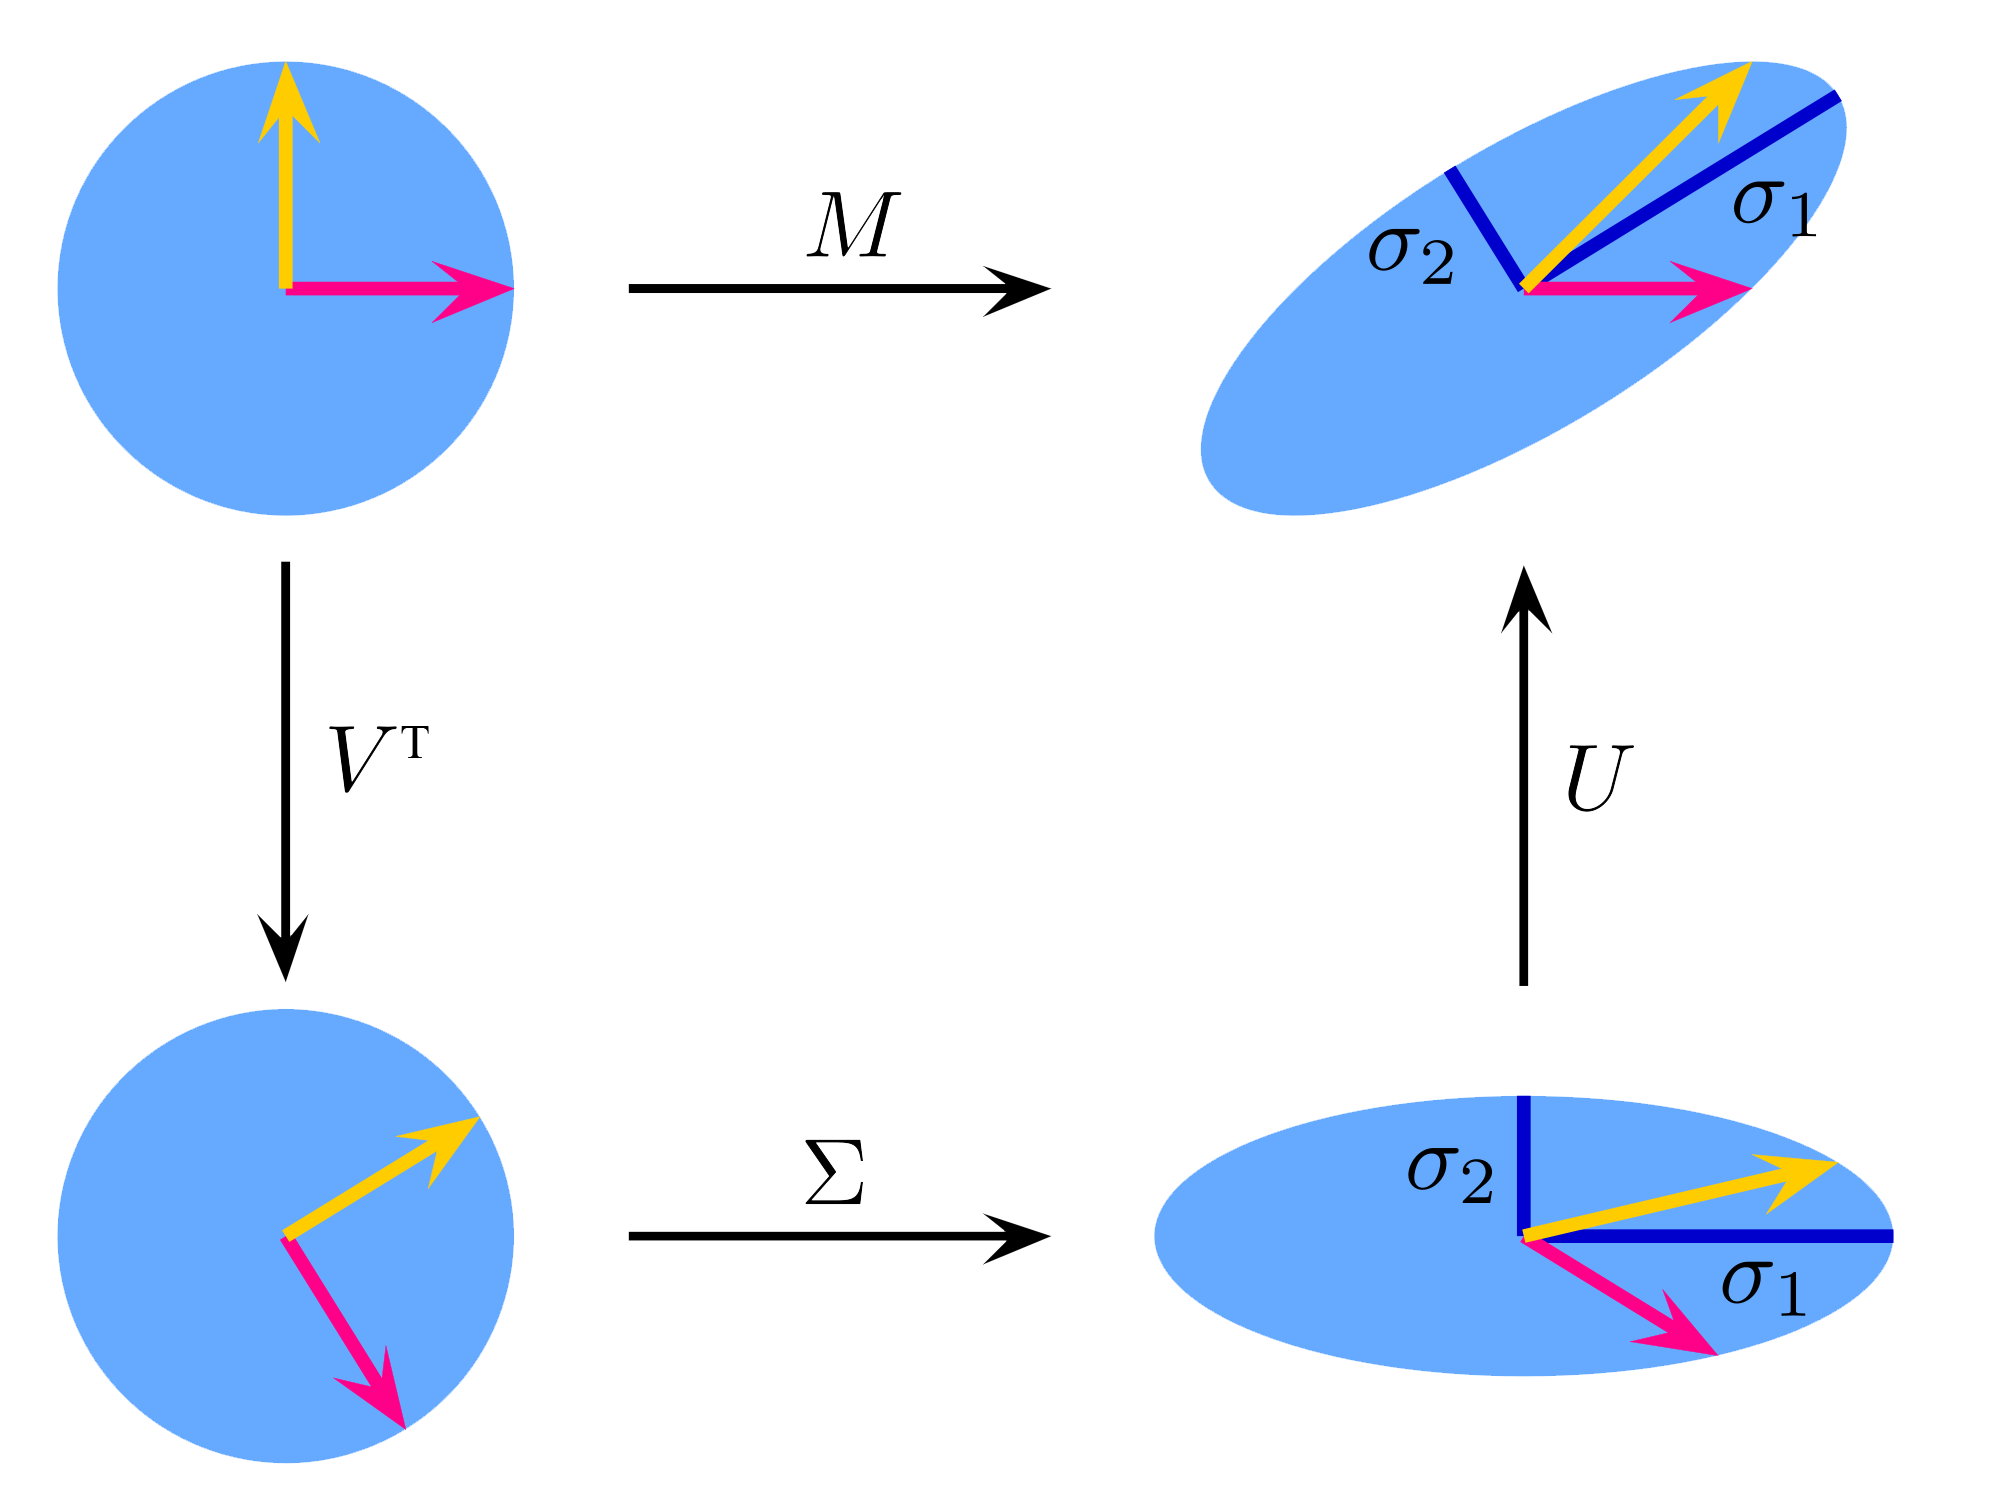
\includegraphics[width=0.65\textwidth]{Chapter7/images/image006.png} 
    \end{center}
\end{frame}




\begin{frame}\frametitle{A Procedure for Constructing the SVD of $A$}
    Suppose $A$ is $m \times n$ and has rank $r$. 
    
    \begin{enumerate}
        \item<2-> Compute the squared singular values of $A^TA$, $\sigma_i^2$, and construct $\Sigma$. \vspace{6pt}
        \item<3-> Compute the unit singular vectors of $A^TA$, $\vec v_i$, use them to form $V$. \vspace{6pt}
        \item<4-> Compute an orthonormal basis for Col$A$ using $$\vec u_i = \frac{1}{\sigma_i}A\vec v_i, \quad i = 1, 2, \ldots r$$ If necessary, extend the set $\{\vec u_i\}$ to form an orthonormal basis for $\mathbb R^m$ and use the basis to form $U$. 
    \end{enumerate}
\end{frame}




\begin{frame}\frametitle{Example}
    Construct the singular value decomposition for $A = 
    \begin{pmatrix}
    2 & 0 \\ 0 & -3 \\ 0 & 0 \\ 0 & 0 
    \end{pmatrix}
    $.
    
    \vspace{12pt}
    \pause 
    \Emph{Solution}\\ \pause 
    Singular values: 
    $$A^TA = \spalignmat{4 0;0 9} \quad \Rightarrow \quad \lambda_1 = 9, \lambda_2=4$$ \pause 
    The positive square roots of the eigenvalues are the singular values. 
    $$\sigma_1 = 3, \ \sigma_2 = 2$$
    \textit{Don't forget that $\sigma_1$ is the largest singular value.}
    
\end{frame}




\begin{frame}\frametitle{Example: Construct $\Sigma$ and $V$}    
    Using the singular values we can construct $\Sigma$. 
    $$\sigma_1 = 3, \ \sigma_2 = 2 \ \Rightarrow \ \Sigma = \spalignmat{3 0;0 2;0 0;0 0}$$
    
    \onslide<2->{Next we construct the right-singular vectors $\{\vec v_i\}$ and form $V$. }
    \begin{align*}
        \onslide<3->{A^TA - \lambda_1 I &= \spalignmat{-5 0;0 0} \quad \Rightarrow \quad \vec v_1 = \spalignmat{0;1}} \\
        \onslide<4->{A^TA - \lambda_2 I &= \spalignmat{-5 0;0 0} \quad \Rightarrow \quad \vec v_2 = \spalignmat{1;0} } \onslide<5->{\quad \Rightarrow \quad
        V = \spalignmat{\vec v_1  \vec v_2} = \spalignmat{0 1;1 0}}
    \end{align*}
\end{frame}




\begin{frame}\frametitle{Example: Construct $\vec u_i$}    
    Next we construct left-singular vectors $\{\vec u_i \}$ using $\vec u_i = \frac{1}{\sigma_i}A\vec v_i$ for $i = 1, 2, \ldots r$. \onslide<2->{Each $\vec u_i$ will be a unit vector in $\mathbb R^4$.}
    \begin{align*}
        \onslide<3->{\vec u_1 &= \frac{1}{\sigma_1}A\vec v_1 = \frac{1}{3}\begin{pmatrix}
    2 & 0 \\ 0 & -3 \\ 0 & 0 \\ 0 & 0 
    \end{pmatrix}\spalignmat{0;1} = \spalignmat{0;-1;0;0}}\\[12pt]
    \onslide<4->{\vec u_2 &= \frac{1}{\sigma_2}A\vec v_2 = \frac{1}{2}\begin{pmatrix}
    2 & 0 \\ 0 & -3 \\ 0 & 0 \\ 0 & 0 
    \end{pmatrix}\spalignmat{1;0} = \spalignmat{1;0;0;0}}
    \end{align*}

\end{frame}




\begin{frame}\frametitle{Example: Construct $U$}  

    To construct the SVD of $A$, we must construct the last two columns of $U$. 
    \begin{itemize}
        \item<2-> In this example, $A$ has rank $r=2$ and $U$ will be a $4 \times 4$ orthogonal matrix.
        \item<3-> Because the columns of $U$ must be orthonormal, and $\vec u_1$ and $\vec u_2$ were standard vectors, by inspection we can set the last two columns to be
        $$\vec u_3 = \spalignmat{0;0;1;0}, \quad \vec u_4 = \spalignmat{0;0;0;1}$$  
        Note that $\vec u_3$ and $\vec u_4$ are unit vectors, and that $\{\vec u_i\}$ are orthonormal. 
        \item<4-> We could have chosen other vectors for $\vec u_3$ and $\vec u_4$.
    \end{itemize}
    
\end{frame}




\begin{frame}\frametitle{Example: Construct $SVD$}  

    We have the SVD of $A$. 
    
    $$A = \begin{pmatrix}
    2 & 0 \\ 0 & -3 \\ 0 & 0 \\ 0 & 0 
    \end{pmatrix}
    = 
    \spalignmat{0 1 0 0;-1 0 0 0;0 0 1 0;0 0 0 1}
    \spalignmat{3 0;0 2;0 0;0 0}
    \spalignmat{0 1;1 0}
    $$
    
\end{frame}







\frame{\frametitle{Summary}

    \SummaryLine \vspace{4pt}
    \begin{itemize}\setlength{\itemsep}{8pt}

        \item the definition of the SVD
        \item computing the SVD for a matrix

    \end{itemize}
    
    \vspace{6pt}
}




